\documentclass[../resumosLPOO.tex]{subfiles}

\newenvironment{conditions}
  {\par\vspace{\abovedisplayskip}\noindent\begin{tabular}{>{$}l<{$} @{${}={}$} l}}
  {\end{tabular}\par\vspace{\belowdisplayskip}}

\begin{document} 

Não é uma linguagem OOP pura, porque as variáveis podem ter valores primitivos ou ser referenciadas como objetos.

Não há apontadores, mas variáveis primitivas são guardadas como valores e objetos são guardados como referências.

Literals: são representações sintáticas de variáveis (Boolean, Character, String, Integer, ...).

Operador == compara tipos primitivos pelo seu valor, mas compara objetos pela sua referência.

Input/Output:
\begin{itemize}
    \item \lstinline{System.out.println(...);}
    \item \lstinline{Scanner scanner = new Scanner(System.in);} \\ \lstinline{String line = scanner.nextLine();} 
\end{itemize}

Strings de Java são imutáveis. Para as comparar usa-se o método equals().

OOP: providencia uma abstração onde os elementos do problema são objetos no espaço solução; permite descrever o problema em termos do problema.

\paragraph{}

Pilares da Orientação por Objetos (A PIE)
\begin{itemize}
    \item Data \textbf{A}bstraction: separação entre interface pública de um tipo de dados e a sua implementação
    \item \textbf{P}olymorphism: um único símbolo pode representar muitos tipos
    \item \textbf{I}nheritance: objetos podem herdar propriedades e comportamentos de outros objetos
    \item \textbf{E}ncapsulation: acesso restrito a algumas componentes de um objeto
\end{itemize}

\paragraph{}

Visibilidade:
\begin{itemize}
    \item Classes:
    \begin{itemize}
        \item public
        \item protected (mesmo package)
        \item private (dentro de outras classes)
    \end{itemize}
    \item Variáveis e Métodos:
    \begin{itemize}
        \item public
        \item protected
        \item private
        \item package
    \end{itemize}
\end{itemize}

\paragraph{}

Para criar um novo objeto é necessário usar new:
\begin{lstlisting}
    Light light = new Light();
    Light another = light;
\end{lstlisting}

\begin{figure}[!h]
    \centering
    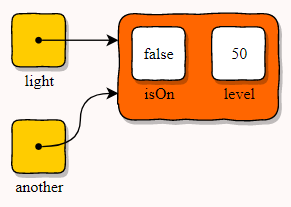
\includegraphics{images/javaNewObject.PNG}
    \caption{Criação de novo objeto}
    \label{fig:javaNew Object}
\end{figure}

\paragraph{}

Para termos duas instâncias do mesmo objeto, a classe tem que implementar a interface Cloneable e o seu método clone();

\paragraph{}

\lstinline{final}: variável que não pode ser alterada.

\paragraph{}

Herança deve ser usada para estabelecer uma relação de is-a (é um/a). Só é possível estender uma classe.

Métodos final, static e private não podem ser reescritos.

Deve-se reescrever o método equals() para todas as classes que vão ser comparadas, o método hashCode() quando usamos HashSet e o método toString().

\paragraph{}

O bloco finally executa sempre que se sai de um bloco try. Assegura que este código é sempre corrido mesmo que ocorra uma exceção.

\begin{lstlisting}
    try {
        ...
    } catch {
        ...
    } finally { ... }
\end{lstlisting}

\paragraph{}

Coleções: Set, List, Queue, Deque, Map
\begin{itemize}
    \item São parameterizadas
    \item Exemplo: \lstinline{List<Animal> list = new ArrayList<>();}
    \begin{itemize}
        \item Princípio "Retorna o tipo mais específico, aceito o tipo mais genérico"
    \end{itemize}
\end{itemize}

\end{document}

